\chapter{LƯA CHỌN PHƯƠNG ÁN}
    \section{Lựa chọn phương án cơ khí}
        \subsection{Yêu cầu phương án cơ khí}
            \begin{itemize}
                \item Đảm bảo độ bám đường, khó lật khi vào cua với tốc độ cao.
                \item Thuật toán điều khiển đơn giản.
                \item Kết cấu cơ khí vững, nhỏ gọn, ổn định và dễ chế tạo.
                \item Chủ động trong việc chuyển hướng, chuyển hướng tốt. 
            \end{itemize}
        \subsection{So sánh các sơ đồ nguyên lý}
            \hspace*{0.6cm}Xét theo từng sơ đồ nguyên lý đã tìm hiểu trong phần tổng quan, bảng dưới đây 
                            trình bày ưu và nhược điểm của từng loại sơ đồ:
            \begin{longtable}{|p{4cm}|p{5cm}|p{5cm}|}
                \caption{So sánh các sơ đồ nguyên lý robot} 
                \label{tab:compare_robot_schemes} \\ 
                \hline
                \textbf{Sơ đồ nguyên lý} & \textbf{Ưu điểm} & \textbf{Nhược điểm} \\
                \hline
                \endfirsthead
                \hline
                \textbf{Sơ đồ nguyên lý} & \textbf{Ưu điểm} & \textbf{Nhược điểm} \\
                \hline
                \endhead
                \hline
                \endfoot
                \hline
                \endlastfoot
                Robot Zumo Slim \newline
                \textit{Phương án 1} \newline
                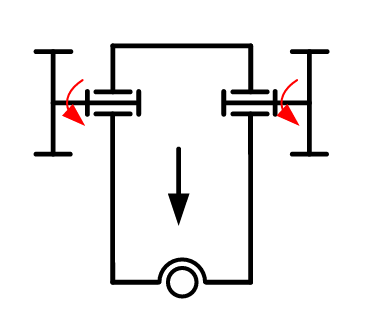
\includegraphics[width=3cm]{pictures/chapter2/chapter2_pic_1.png} & 
                - Kết cấu 3 bánh nhỏ gọn, đơn giản \newline
                - Mô hình toán đơn giản, dễ điều khiển \newline
                - Đảm bảo xe luôn được đồng phẳng & 
                - Khả năng bám đường không tốt, vào cua ở tốc độ cao dễ bị trượt. \newline
                - 2 bánh sau vừa dẫn động vừa dẫn hướng, trọng tâm không nằm trên trục bánh sau dẫn tới dễ bốc đầu khi chạy ở tốc độ cao. \\
                \hline
                Robot Pinto \newline
                \textit{Phương án 2} \newline
                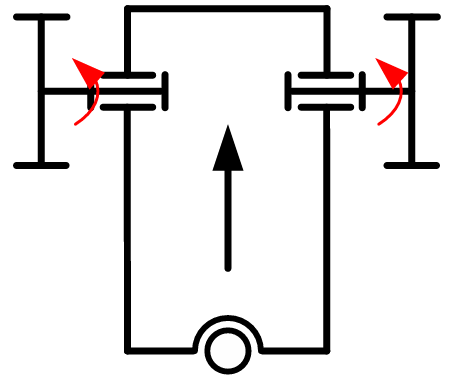
\includegraphics[width=3cm]{pictures/chapter2/chapter2_pic_2.png} & 
                - Kết cấu 3 bánh nhỏ gọn, đơn giản \newline
                - Mô hình toán đơn giản, dễ điều khiển \newline
                - Đảm bảo xe luôn được đồng phẳng & 
                - Khả năng bám đường không tốt, vào cua ở tốc độ cao dễ bị trượt. \newline
                - Do dẫn động nằm phía trước nên giảm thời gian phản ứng khi dò line. \\
                \hline
                Robot Newbie \newline
                \textit{Phương án 3} \newline
                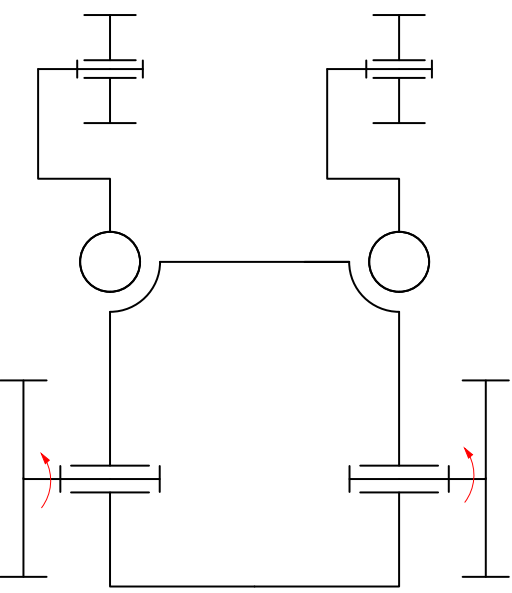
\includegraphics[width=2.5cm]{pictures/chapter2/chapter2_pic_3.png} & 
                - Kết cấu 4 bánh giúp tăng khả năng tải. \newline
                - Khả năng vào cua và bám đường tốt. \newline
                - Kết cấu cơ khí đơn giản & 
                - Đảm bảo đồng trục 2 bánh dẫn động. \newline
                - Đảm bảo đồng phẳng giữa các bánh xe. \newline
                - Bị hóc đầu nếu đặt tải lệch về phía sau. \newline
                - Dễ bị lật khi vào cua với tốc độ cao. \newline
                - Mô hình tính toán phức tạp, khó điều khiển. \\
                \hline
                Robot FireBall \newline
                \textit{Phương án 4} \newline
                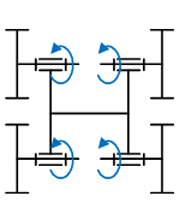
\includegraphics[width=2.5cm]{pictures/chapter2/chapter2_pic_4.png} &
                - Kết cấu cơ khí đơn giản, cân bằng tốt. \newline
                - Tải chia đều cho 4 động cơ -> giảm tải. \newline
                - Điều khiển tùy ý dễ dàng. &
                - Đảm bảo đồng trục cả 2 bánh trước và 2 bánh sau. \newline
                - Đảm bảo đồng phẳng giữa các bánh. \newline
                - Mô hình tính toán phức tạp, khó điều khiển. \\ 
                \hline
                Robot Khepera IV \newline
                \textit{Phương án 5} \newline
                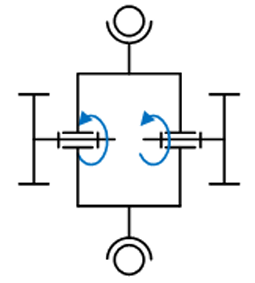
\includegraphics[width=2.5cm]{pictures/chapter2/chapter2_pic_5.png} &
                - Kết cấu 4 bánh đơn giản, mô hình toán đơn giản, dễ điều khiển.\newline 
                - Trọng tâm nằm ngay trục dẫn động giữ kết cấu dễ ổn định. &
                - Khả năng vào cua kém. \newline
                - Đảm bảo đồng trục giữa 2 bánh dẫn động và đồng phẳng giữa các bánh. \newline
                - Hai bánh giữa chịu áp lực lớn vừa chịu tải vừa kéo tải. \\
                \hline
                
            \end{longtable}
        \subsection{Số bánh}
            \begin{longtable}{|p{4cm}|p{5cm}|p{5cm}|}
                \caption{So sánh số lượng bánh xe robot} 
                \label{tab:compare_robot_wheels} \\ 
                \hline
                \textbf{Số bánh} & \textbf{Ba bánh} & \textbf{Bốn bánh} \\
                \hline
                \endfirsthead
                \hline
                \textbf{Số bánh} & \textbf{Ba bánh} & \textbf{Bốn bánh} \\
                \hline
                \endhead
                \hline
                \endfoot
                \hline
                \endlastfoot
                \textbf{Ưu điểm} &
                - Yêu cầu về đồng phằng đáp ứng dễ dàng. \newline
                - Mô hình xe có kết cấu đơn giản. &
                - Khả năng bám đường tốt, khả năng ít bị lật khi vào cua. \newline
                - Khi sử dụng vi sai thì vấn đề đồng trục hai bánh sau có thể được bỏ qua. \\
                \hline
                \textbf{Nhược điểm} &
                - Khả năng bám đường không tốt, khi vào cua dễ bị lật. \newline
                - Phải đảm bảo hai bánh sau đồng trục để thỏa yêu cầu xe chạy không đảo, lắc. &
                - Mô hình xe có kết cấu phức tạp (nhất là khi sử dụng vi sai). \newline 
                - Phải đảm bảo đồng phẳng cho cả bốn bánh. \\ 
            \end{longtable}
        \subsection{Vật liệu}
            \begin{table}[H]
                \centering
                \begin{tabular}{|c|p{2.8cm}|p{2.8cm}|p{2.8cm}|p{2.8cm}|}
                    \hline
                    \textbf{Vật liệu} & \textbf{Gỗ} & \textbf{Mica} & \textbf{Nhôm} & \textbf{Inox} \\
                    \hline
                    \textbf{Ưu điểm} 
                    & Nhẹ nhất trong 3 loại vật liệu được liệt kê, dễ dàng gia công, không dẫn điện, an toàn, không gây chập mạch.  
                    & Chịu được ẩm, chịu được nhiệt độ cao, chịu được lực, không dẫn điện không gây chập mạch, dễ gia công.
                    & Độ bền cao, chắc chắn, nhẹ hơn so với các kim loại khác, có thể sơn phủ để tăng tính thẩm mĩ.
                    & Độ bền cao, chắc chắn. \\
                    \hline
                    \textbf{Nhược điểm} 
                    & Dễ bị tác động bởi môi trường, khả năng chống va đập thấp.
                    & Dễ trầy xước.
                    & Giá thành gia công cao.
                    & Giá thành gia công cao. \\
                    \hline
                \end{tabular}
                \caption{So sánh các loại vật liệu chế tạo robot}
                \label{tab:label}
            \end{table}
        \hspace*{0.6cm}\textbf{Kết luận}: sau khi phân tích các phương án kết cấu cơ khí cùng với yêu cầu được đặt ra về vận tốc không cao, không phải chịu tải nặng. Nhóm quyết định xe 3 bánh, 2 bánh dẫn động ở phía trước và 1 bánh dẫn hướng phía sau để đảm bảo đồng phẳng và dễ điều khiển theo cơ cấu Pinto. Vật liệu được nhóm lựa chọn để thiết kế khung xe với yêu cầu kỹ thuật trên là nhôm với độ dày 2mm. 
    \section{Lựa chọn phương án điện}
        \subsection{Lựa chọn cảm biến dò line}
            \subsubsection{Yêu cầu cảm biến}
                \begin{itemize}
                    \item Đáp ứng nhanh khi nhận biết sự thay đổi màu sắc giữa trắng và đen trên sa bàn.
                    \item Tín hiệu cảm biến trả về nhanh để giúp xe kịp thời chuyển hướng ở những đoạn line uốn cong.
                    \item Tín hiệu đọc về dạng analog, ít nhiễu. Giải thuật đơn giản.
                    \item Dễ tìm thấy trên thị trường, giá thành hợp lý. 
                \end{itemize}
            \subsubsection{So sánh các loại cảm biến}
                \begin{table}[H]
                    \centering
                    \begin{tabular}{|>{\raggedright\arraybackslash}p{2.5cm}|>{\raggedright\arraybackslash}p{3cm}|>{\raggedright\arraybackslash}p{4cm}|>{\raggedright\arraybackslash}p{3cm}|}
                    \hline
                    \textbf{Loại cảm biến} & \textbf{Camera} & \textbf{Cảm biến hồng ngoại} & \textbf{Cảm biến quang trở} \\
                    \hline
                    \textbf{Dạng tín hiệu} & Digital image & Analog và digital & Digital \\
                    \hline
                    \textbf{Độ phức tạp điều khiển} & Phức tạp do phải sử dụng thuật toán xử lí ảnh để tìm ra góc lệch của xe so với đường thẳng. & Đơn giản khi sử dụng tín hiệu digital. & Đơn giản. \\
                    \hline
                    \textbf{Xử lí nhiễu} & Xử lí bằng chương trình. & Có thể xử lí bằng kết cấu cơ khí và che chắn phù hợp. & Có thể xử lí bằng kết cấu cơ khí và che chắn phù hợp. \\
                    \hline
                    \multirow{3}{*}{\textbf{Ưu điểm}} & Độ chính xác cao, có thể tận dụng dễ dàng để làm đa tác vụ thay cho nhiều cảm biến. & Nhỏ gọn, rẻ, dễ dùng. Độ chính xác cao, có thể tận dụng để làm đa tác vụ thay cho nhiều cảm biến.\newline Nhận diện được line có độ tương phản cao. & Nhỏ gọn, rẻ để sử dụng. \\
                    \hline
                    \multirow{3}{*}{\textbf{Nhược điểm}} & Giá thành tương đối cao.\newline Cần thời gian để xử lí thuật toán trên ảnh nên phải đi kèm với khi xử lí mạnh.\newline Khó gá đặt. & Khoảng cách nhận biết có giới hạn nên cần gá đặt ở vị trí phù hợp. \newline Nhạy với nhiễu. & Nhạy cảm với ánh sáng môi trường. \newline Nhạy với nhiễu. \\
                    \hline
                    \end{tabular}
                \end{table}
            \subsubsection{Kết luận}
                \hspace*{0.6cm}Sau khi phân tích về ưu nhược điểm của ba phương án cảm biến dò line ở chương 
                                1, nhóm quyết định lựa chọn cảm biến IR TCRT5000, đồng thời thiết kế mạch PCB có 
                                tính toán số lượng cảm biến, khoảng cách giữa các cảm biến và độ cao gá đặt cảm biến tới mặt line.
            \subsubsection{Cảm biến hồng ngoại TCRT5000}
                \begin{figure}[H]
                    \centering
                    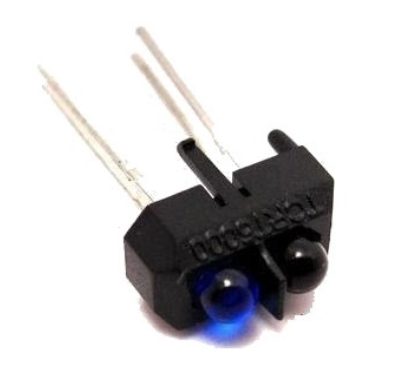
\includegraphics[width=0.25\textwidth]{pictures/chapter2/chapter2_pic_6.png}
                    \caption{Cảm biến hồng ngoại TCRT5000}
                    \label{fig:tcrt5000}
                \end{figure}
                \hspace*{0.6cm}Cảm biến hồng ngoại TCRT5000 là cảm biến quang điện có khả năng phát hiện vật thể dựa trên sự phản xạ của ánh sáng hồng ngoại. Cảm biến này bao gồm một LED hồng ngoại và một phototransistor, cho phép nó phát hiện sự hiện diện của vật thể trong khoảng cách từ 0 đến 25 cm. 
        \subsection{Phương án bố trí cảm biến dò line}
            \subsubsection{Các phương án bố trí cảm biến}
                \begin{itemize}
                    \item Bố trí dạng ma trận:
                    \begin{figure}[H]
                        \centering
                        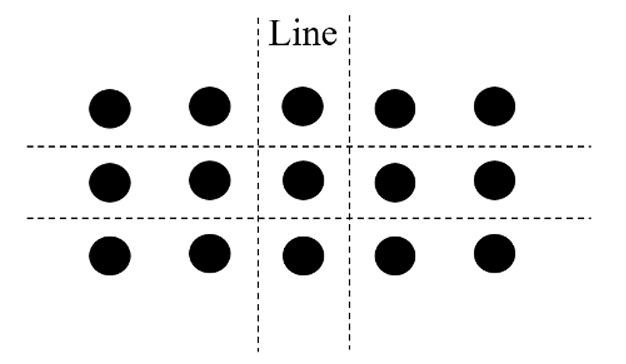
\includegraphics[width=0.5\textwidth]{pictures/chapter2/chapter2_pic_7.png}
                        \caption{Bố trí cảm biến dạng ma trận}
                        \label{fig:matrix_sensor_layout}
                    \end{figure}
                    \item Bố trị dạng đường thẳng:
                    \begin{figure}[H]
                        \centering
                        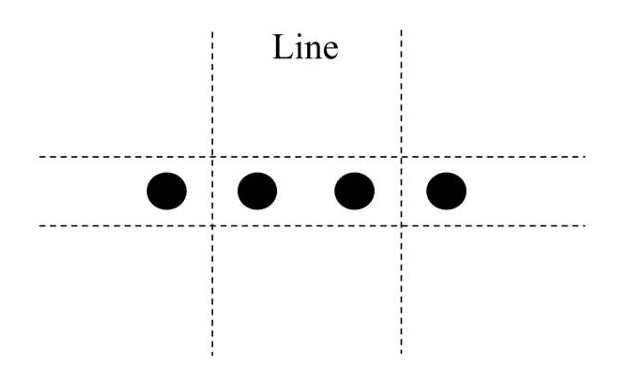
\includegraphics[width=0.5\textwidth]{pictures/chapter2/chapter2_pic_8.png}
                        \caption{Bố trí cảm biến dạng đường thẳng}
                        \label{fig:line_sensor_layout}
                    \end{figure}
                    \item Bố trí dạng chữ V:
                    \begin{figure}[H]
                        \centering
                        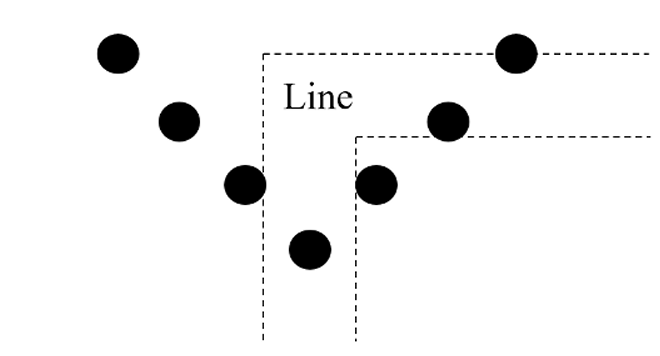
\includegraphics[width=0.5\textwidth]{pictures/chapter2/chapter2_pic_9.png}
                        \caption{Bố trí cảm biến dạng chữ V}
                        \label{fig:v_sensor_layout}
                    \end{figure}
                \end{itemize}
                \begin{table}[H]
                    \centering
                    \begin{tabular}{|p{3cm}|p{5cm}|p{5cm}|}
                        \hline
                        \textbf{Dạng bố trí} & \textbf{Ưu điểm} & \textbf{Nhược điểm} \\
                        \hline
                        \textbf{Dạng ma trận} &
                        - Thu được nhiều thông tin để nội suy hay so sánh làm tăng độ chính xác. \newline
                        - Có thể dự đoán trước được đường đi. &
                        - Sử dụng nhiều cảm biến. \newline
                        - Khối lượng xử lý lớn, thuật toán xử lý phức tạp. \\ 
                        \hline
                        \textbf{Dạng đường thẳng} &
                        - Thuật toán đơn giản.  \newline
                        - Phát hiện được các đoạn giao. \newline
                        - Được sử dụng phổ biến.  &
                        - Xử lý những đoạn cua gắt kém. \\
                        \hline
                        \textbf{Dạng chữ V} &
                        - Thích hợp cho đường line có nhiều đoạn cua gắt (lớn hơn 90 độ). &
                        - Ít được sử dụng phổ biến. \newline
                        - Giải thuật xử lý phức tạp hơn so với dạng đường thẳng. \\ 
                        \hline
                    \end{tabular}
                    \caption{Mô tả bảng}
                    \label{tab:label}
                \end{table}
            \subsubsection{Kết luận}
                \hspace*{0.6cm}Với sa bàn được yêu cầu trên đầu bài, bề rộng line là 26 mm với các khúc cua đơn giản, không phức tạp, nhóm lựa chọn bố trí cảm biến theo dạng đường thẳng. 
        \subsection{Lựa chọn giải thuật xác định tọa độ line}
            \subsubsection{Các giải thuật xác định tọa độ line}
                \begin{itemize}
                    \item Giải thuật ngưỡng nhị phân (Binary Thresholding):
                        Đọc giá trị cảm biến và so sánh với ngưỡng, chỉ phân biệt "có line" hoặc "không có line" bằng cách so sánh giá trị cảm biến với một ngưỡng cố định. Nếu giá trị cảm biến vượt ngưỡng thì coi như phát hiện line, ngược lại thì không có line. 
                    \item Giải thuật trung bình có trọng số (Weighted Average):
                        Tính toán vị trí chính xác của line bằng cách coi giá trị các cảm biến như "trọng số" và vị trí của chúng như "tọa độ". Vị trí line được xác định bằng cách tính trung bình có trọng số của tất cả các cảm biến, trong đó cảm biến nào có giá trị cao hơn sẽ có ảnh hưởng lớn hơn đến kết quả cuối cùng.
                    \item Giải thuật phát hiện cạnh (Edge Detection):
                        Tìm kiếm các cạnh biên của line thay vì tìm trung tâm trực tiếp. Nó phát hiện những điểm có sự thay đổi mạnh về cường độ tín hiệu giữa các cảm biến liền kề để xác định cạnh trái và cạnh phải của line, sau đó tính toán vị trí trung tâm line dựa trên hai cạnh này.
                \end{itemize}
                \begin{table}[H]
                    \centering
                    \caption{So sánh các giải thuật dò line chính}
                    \begin{tabular}{|p{3cm}|p{3.75cm}|p{3.75cm}|p{3.75cm}|}
                        \hline
                        \textbf{Tiêu chí} & \textbf{Binary Threshold} & \textbf{Weighted Average} & \textbf{Edge Detection} \\
                        \hline
                        \textbf{Tốc độ xử lý} & Nhanh nhất & Nhanh & Trung bình \\
                        \hline
                        \textbf{Độ phức tạp} & Đơn giản nhất & Trung bình & Phức tạp nhất \\
                        \hline
                        \textbf{Độ chính xác} & Thấp & Cao nhất & Cao \\
                        \hline
                        \textbf{Chống nhiễu} & Yếu & Tốt & Rất tốt \\
                        \hline
                        \textbf{Tính ổn định} & Kém & Rất tốt & Tốt \\
                        \hline
                        \textbf{Bộ nhớ cần} & Ít nhất & Trung bình & Nhiều nhất \\
                        \hline
                        \textbf{Phù hợp MCU} & 8-bit & 16/32-bit & 32-bit \\
                        \hline
                    \end{tabular}
                    \label{tab:comparison}
                \end{table}
            \subsubsection{Kết luận}
                \hspace*{0.6cm}Sau khi phân tích các giải thuật dò line, nhóm quyết định sử dụng giải thuật trung bình có trọng số (Weighted Average) để xác định tọa độ line do tốc độ xử lý nhanh và độ chính xác cao cũng như ổn định trong các giải thuật dò line phổ biến.
        \subsection{Lựa chọn số lượng cảm biến}
            \hspace*{0.6cm}Để sử dụng giải thuật trung bình trọng số cần dùng ít nhất 3 cảm biến để nhận dạng tâm đường line (1 cảm biến để tham chiếu vị trí trung tâm và 2 cảm biến để nhận diện lệch). Tuy nhiên để tăng tầm phát hiện khi robot lệch xa khỏi line cũng như phát hiện ngã rẻ, ta cần thêm 1 cảm biến ở mỗi bên. Do đó nhóm quyết định sử dụng 5 cảm biến. 
    \subsection{Lựa chọn cảm biến màu sắc}
        \subsubsection{Yêu cầu cảm biến màu sắc}
            \begin{itemize}
                \item Nhận biết được hai màu đỏ và xanh.
                \item Giá thành phù hợp và dễ dàng tìm thấy trên thị trường. 
                \item Nhỏ gọn để dễ dàng bố trí trên xe. 
                \item Giải thuật xử lý đơn giản.
            \end{itemize}
        \subsection{So sánh các cảm biến màu sắc}
            \newpage
            \begin{table}[h!]
                \centering
                \begin{tabular}{|>{\raggedright\arraybackslash}p{4cm}|>{\raggedright\arraybackslash}p{5.5cm}|>{\raggedright\arraybackslash}p{5.5cm}|}
                \hline
                \textbf{Tiêu chí} & \textbf{Cảm biến màu sắc} & \textbf{Camera} \\
                \hline
                \textbf{Ưu điểm} 
                & 
                - Nhỏ gọn, dễ tích hợp \newline
                - Giá thành thấp \newline
                - Dễ sử dụng với vi điều khiển \newline
                - Tốc độ phản hồi nhanh
                &
                - Nhận diện được nhiều vùng màu cùng lúc \newline
                - Phân tích màu theo vị trí và hình dạng \newline
                - Độ chính xác cao \newline
                \\
                \hline
                \textbf{Nhược điểm} 
                & 
                - Chỉ nhận diện được màu sắc của 1 vật vào 1 thời điểm \newline
                - Phụ thuộc điều kiện ánh sáng môi trường \newline
                &
                - Chi phí cao \newline
                - Thuật toán xử lý phức tạp \newline
                - Tốc độ xử lý có thể chậm hơn
                \\
                \hline
                \end{tabular}
                \caption{So sánh cảm biến màu sắc và camera trong nhận diện màu sắc}
            \end{table}
        \subsubsection{Kết luận}
            \hspace*{0.6cm}Dựa vào bảng so sánh, nhóm lựa chọn cảm biến màu sắc do đáp ứng đủ tiêu chí đề ra. Thông qua tìm hiểu trên thị trường, nhóm chọn sản phẩm TCS3200D. 
        \subsubsection{Cảm biến màu sắc TCS3200}
            \begin{figure}[H]
                \centering
                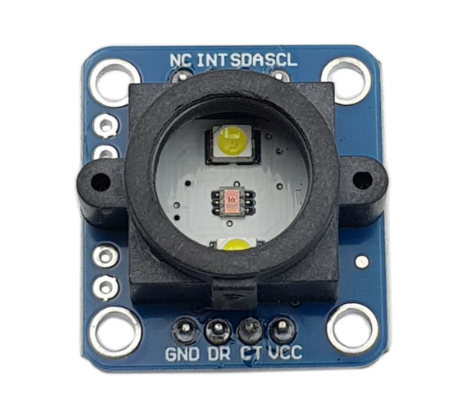
\includegraphics[width=0.25\textwidth]{pictures/chapter2/chapter2_pic_10.png}
                \caption{Cảm biến màu sắc TCS3200}
                \label{fig:tcs3200}
            \end{figure}
            \hspace*{0.6cm}Cảm biến TCS3200 là cảm biến màu sắc có khả năng phát hiện và phân tích màu sắc của vật thể bằng cách sử dụng các bộ lọc màu đỏ, xanh lá cây và xanh dương. Nó cung cấp tín hiệu đầu ra dạng tần số tương ứng với cường độ của từng màu sắc, cho phép xác định màu sắc của vật thể một cách chính xác.
        \subsection{Lựa chọn vi điều khiển}
            \subsection{Yêu cầu vi điều khiển}
                \begin{itemize}
                    \item Có ít nhất 5 kênh ADC để đọc giá trị analog từ cảm biến dò line. 
                    \item Có ít nhất 2 timer tốc độ cao và hai chân ngắt ngoài để đọc encoder trả về từ động cơ. 
                    \item Cần ít nhất 1 timer để tạo xung PWM cho hai động cơ. 
                    \item Tốc độ xử lý nhanh để bảo đảm thực hiện các tác vụ nhanh.
                    \item Giá thành hợp lý, dễ dàng tìm thấy trên thị trường. 
                \end{itemize}
            \subsection{So sánh các vi điều khiển}
            \begin{table}[H]
                \centering
                \begin{tabular}{|p{2.5cm}|>{\raggedright\arraybackslash}p{3.8cm}|>{\raggedright\arraybackslash}p{3.8cm}|>{\raggedright\arraybackslash}p{3.8cm}|}
                    \hline
                    \textbf{Dòng VDK} & \textbf{STM32F103C8T6} & \textbf{Microchip PIC16F887} & \textbf{ATMega328p} \\
                    \hline
                    \textbf{Tần số hoạt động tối đa} & 72 MHz & 20 MHz & 16MHz \\
                    \hline
                    \textbf{Tổng chân I/O} & 32 & 35 & 14 \\
                    \hline
                    \textbf{Timer} & \makecell[l]{4 bộ 16 bit} & \makecell[l]{1 bộ 8 bit và\\2 bộ 16 bit} & \makecell[l]{2 bộ 8 bit và\\1 bộ 16 bit} \\
                    \hline
                    \textbf{Giao tiếp} & \makecell[l]{2×I2C, 2×SPI,\\3×UART, 1×CAN,\\1×USB2.0} & \makecell[l]{1×I2C, 1×SPI,\\1×UART} & \makecell[l]{1×I2C, 1×SPI,\\1×UART} \\
                    \hline
                    \textbf{Số kênh ADC} & 10 kênh & 14 kênh & 6 kênh \\
                    \hline
                    \textbf{Giá thành (VND)} & 60.000 - 100.000 & 69.000 - 100.000 & 150.000 - 250.000 \\
                    \hline
                    \textbf{PWM} & 15 chân PWM 16 bit & 2 khối PWM, 10 bit & 6 chân PWM 8 bit \\
                    \hline
                \end{tabular}
                \caption{So sánh các vi điều khiển phổ biến}
                \label{tab:compare_microcontrollers}
            \end{table}
            \subsection{Kết luận}
                \hspace*{0.6cm}Sau khi phân tích các vi điều khiển, nhóm quyết định sử dụng vi điều khiển STM32F103C8T6 do đáp ứng đủ các yêu cầu về tốc độ xử lý, số lượng chân I/O, số kênh ADC, thư viện HAL sử dụng đơn giản, nhỏ gọn, dễ lắp đặt và giá thành hợp lý. 

        \subsection{Lựa chọn động cơ}
            \subsubsection{Yêu cầu động cơ}
                \begin{itemize}
                    \item Kích thước nhỏ gọn, phù hợp với kết cấu xe.
                    \item Đảm bảo được vận tốc đầu bài đề ra.
                    \item Có momen xoắn đủ lớn để xe có thể di chuyển cùng với vật nặng 1-2 kg.
                \end{itemize}
            \subsection{Kết luận}
                \hspace*{0.6cm}Sau khi phân tích các loại động cơ, nhóm quyết định sử dụng động cơ DC encoder với hộp số (các thông số sẽ được tính sau) để đảm bảo yêu cầu đề ra.
                \begin{figure}[H]
                    \centering
                    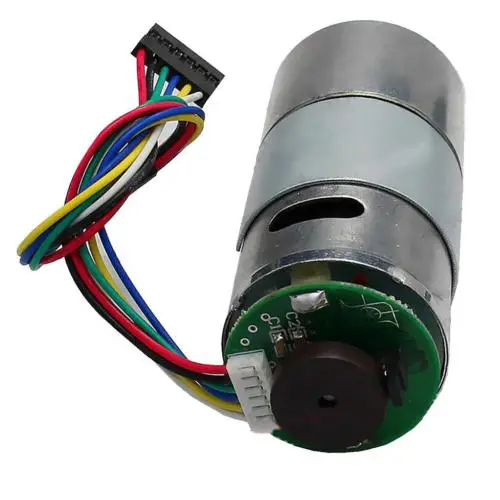
\includegraphics[width=0.25\textwidth]{pictures/chapter2/chapter2_pic_11.png}
                    \caption{Động cơ DC encoder với hộp số}
                    \label{fig:dc_motor_with_encoder}
                \end{figure} 
        \subsection{Lựa chọn mạch điều khiển động cơ}
            \subsubsection{Yêu cầu mạch điều khiển động cơ}
                \begin{itemize}
                    \item Tần số hoạt động đủ lớn, đáp ứng được xung điều khiển.
                    \item Dòng điện ngõ ra phải đảm bảo cung cấp dòng cho hai động cơ.
                    \item Áp đầu ra: Đảm bảo đủ áp cung cấp cho mỗi động cơ là 12V. 
                    \item Đồ thị đáp ứng tuyến tính: đảm bảo độ tương quan giữa xung PWM đầu vào và điện áp cung cấp cho mỗi động cơ đầu ra. 
                \end{itemize}
            \subsubsection{So sánh các mạch điều khiển động cơ về các thông số}
                \begin{table}[H]
                    \centering
                    \begin{tabular}{|p{3cm}|p{4cm}|p{4cm}|}
                        \hline
                        \textbf{Tiêu chí} & \textbf{Mạch L298N} & \textbf{Mạch TB6612FNG} \\
                        \hline
                        \textbf{Điện áp} & 5-46V & 2.7-13.5V \\
                        \hline
                        \textbf{Dòng điện} & 2A mỗi kênh (4A với cầu H) & 1.2A mỗi kênh (3A đỉnh) \\
                        \hline
                        \textbf{Hiệu suất} & Thấp, tiêu thụ năng lượng lớn & Cao, tiết kiệm năng lượng \\
                        \hline
                        \textbf{Tần số PWM} & 25 kHz & 100 kHz \\
                        \hline
                        \textbf{Kích thước} & Lớn & Nhỏ gọn \\
                        \hline
                        \textbf{Tản nhiệt} & Nóng, cần tản nhiệt khi tải cao & Ít nóng, phù hợp xe nhẹ \\
                        \hline
                        \textbf{Độ chính xác} & Phản hồi chậm hơn ở tốc độ cao & Phản hồi nhanh, điều khiển chính xác \\
                        \hline
                        \textbf{Giá thành} & Rẻ& Đắt hơn \\
                        \hline
                        \end{tabular}
                    \caption{So sánh mạch điều khiển động cơ L298N và TB6612FNG}
                    \label{tab:compare_motor_driver}
                \end{table}
            \subsubsection{So sánh các mạnh điều khiển động cơ về đồ thị đáp ứng giữa tốc tốc độ động cơ và tần số xung PWM}
                \begin{figure}[H]
                    \centering
                    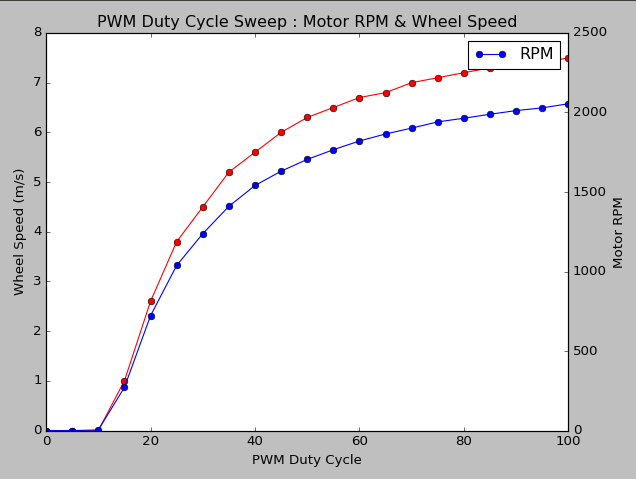
\includegraphics[width=0.6\textwidth]{pictures/chapter2/chapter2_pic_12.png}
                    \caption{Đồ thị đáp ứng của mạch L298N}
                    \label{fig:l298n_response}
                \end{figure}
                \begin{figure}[H]
                    \centering
                    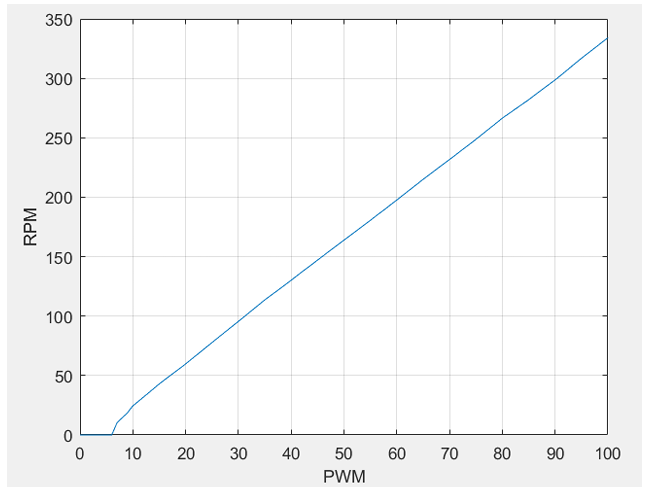
\includegraphics[width=0.6\textwidth]{pictures/chapter2/chapter2_pic_13.png}
                    \caption{Đồ thị đáp ứng của mạch TB6612FNG}
                    \label{fig:tb6612fng_response}
                \end{figure}
            \subsubsection{Kết luận}
                \hspace*{0.6cm}Sau khi phân tích các tiêu chí so sánh, nhóm quyết định sử dụng mạch TB6612 để điều khiển động cơ do đáp ứng được yêu cầu về kích thước nhỏ gọn, hiệu suất cao và độ tuyến tính cao giữa xung PWM và tốc độ quay của động cơ trong điều khiển động cơ.
        \section{Lựa chọn phương án điều khiển}
            \subsection{Lựa chọn cấu trúc điều khiển}
                \subsubsection{Yêu cầu cấu trúc điều khiển}
                    \begin{itemize}
                        \item Dễ dàng quản lý được chương trình. 
                        \item Tiết kiệm được thời gian lập trình. 
                        \item Dễ dàng phân chia công việc cho từng thành viên trong nhóm.
                        \item Chi phí hợp lý. 
                    \end{itemize}
                \subsubsection{So sánh các cấu trúc điều khiển}
                \begin{table}[H]
                    \centering
                    \begin{tabular}{|p{3cm}|p{4cm}|p{4cm}|}
                        \hline
                        \textbf{Cấu trúc} & \textbf{Ưu điểm} & \textbf{Nhược điểm} \\
                        \hline
                        \textbf{Cấu trúc điều khiển tập trung} & 
                        - Tiết kiệm được chi phí và không gian bố trí, giảm khối lượng hệ thống.\newline
                        - Không cần thực hiện giao tiếp giữa các vi điều khiển. & 
                        - Vi điều khiển phải đủ các port I/O, analog, digital, tốc độ xử lý cần thiết. \newline
                        - Khi phát sinh lỗi chương trình, rất khó khăn trong việc tìm kiếm lỗi và sửa lỗi.  \\ 
                        \hline
                        \textbf{Cấu trúc điều khiển phân cấp} & 
                        - Có tính linh hoạt cao trong việc quản lý, mở rộng và sửa chữa. \newline
                        - Dễ dàng tìm kiếm và sửa chữa khi gặp lỗi \newline
                        - Tín hiệu được chia ra và xử lý bất đồng bộ, giúp tiết kiệm thời gian, cũng như giảm dung lượng xử lý cho mỗi vi điều khiển. & 
                        - Tốn thêm chi phí và không gian bố trí vi điều khiển. \\
                        \hline
                        \end{tabular}
                    \caption{So sánh các cấu trúc điều khiển}
                    \label{tab:compare_control_structures}  
                \end{table}
                \subsubsection{Kết luận}
                    \hspace*{0.6cm}Sau khi phân tích các cấu trúc điều khiển, nhóm quyết định sử dụng cấu trúc điều khiển tập trung do đáp ứng được yêu cầu về chi phí, không gian bố trí và dễ dàng quản lý chương trình.
            \subsection{Lựa chọn phương án điều khiển}
            Các phương án lựa chọn cho bài toán bám line
                \subsubsection{Bộ điều khiển fuzzy}
                    \begin{itemize}
                        \item Ưu điểm: Không cần quan tâm về các phương trình của hệ thống, tùy chỉnh trong quá trình hoạt động.
                        \item Nhược điểm: Thiết kế phức tạp, cần có hiểu biết về hệ, có kinh nghiệm về đưa ra được những thông số tối ưu cho hệ.
                    \end{itemize}
                \subsubsection{Bộ điều khiển bám line theo tiêu chuẩn Lyapunov}
                    \begin{itemize}
                        \item Ưu điểm: Áp dụng được cho hệ phi tuyến.
                        \item Nhược điểm: Không tối ưu được các yêu cầu về hiệu suất vì chỉ tập trung vào ổn định.
                    \end{itemize}
                \subsubsection{Bộ điều khiển PID}
                    \begin{itemize}
                        \item Ưu điểm: Đơn giản, dễ hiệu chỉnh.
                        \item Nhược điểm: Áp dụng cho hệ SISO, cần tuyến tính hóa nếu hệ phi tuyến trước khi áp dụng.
                    \end{itemize}
                \subsubsection{Kết luận:} 
                \hspace{0.6cm}Với vận tốc trung bình của xe đặt ra là 0.5 m/s, vận tốc không quá cao, với yêu cầu điều khiển bám line nhóm quyết định sử dụng bộ điều khiển PID làm bộ điều khiển bám line.
                \begin{figure}[H]
                    \centering
                    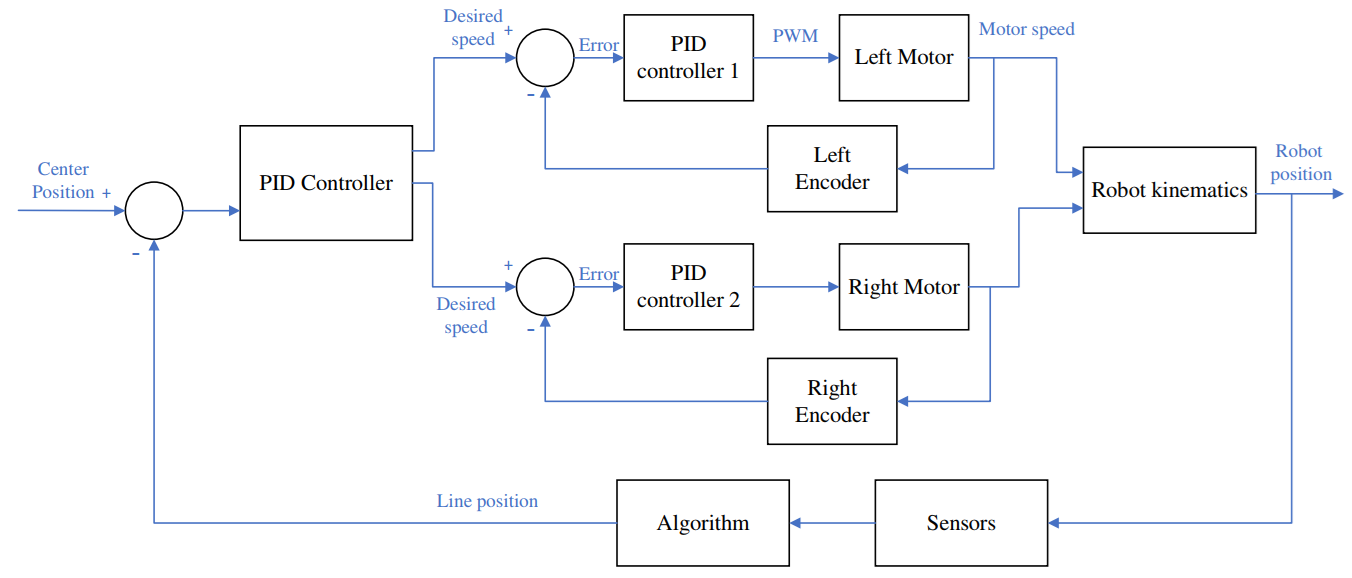
\includegraphics[width=0.8\textwidth]{pictures/chapter2/chapter2_pic_14.png}
                    \caption{Sơ đồ nguyên lý điều khiển}
                    \label{control_principle}
                \end{figure}
                